\chapter{Deep Learning}
\thispagestyle{fancy}
\label{chap:Deep Learning}

Notizen:
\begin{itemize}
	\item Quelle: \cite{ZHA20}
	\item Deep Learning definieren
	\item Machine Learning erwähnen
	\item Siehe Abstract im Exposé
	\item ATS on GitHub: \url{https://github.com/mathsyouth/awesome-text-summarization#corpus}
\end{itemize}


\section{Neuronale Netze}
Notizen:
\begin{itemize}
	\item Neuronale Netze definieren
	\item Historie beschreiben
	\item Funktionsweise und ausgewählte Komponenten beschreiben
\end{itemize}


\section{Architekturen}
Notizen:
\begin{itemize}
	\item Existenz und Notwendigkeit verschiedener Architekturen ankündigen, ggf. in spätere Kapitel verlegen, bspw. zum abstraktiven Ansatz
	\item Später benötigte Architekturen hier beschreiben
	\item Diversität der existierenden Architekturen (wie im Forschungsstand bereits erwähnt) hervorheben
	\item "Reinforcement Learning comes to the rescue" aus \url{https://towardsdatascience.com/deep-learning-models-for-automatic-summarization-4c2b89f2a9ea} einbinden
	\item Encoder/ Decoder, Self-Attention, Seq to Seq, Transformer Model (Recherche + Vergleich)
	\item Transformer, bestehend aus Seq-to-Seq-Model mit Encoder-/ Decoder-Architektur, gut erklärt: \url{https://medium.com/inside-machine-learning/what-is-a-transformer-d07dd1fbec04}, wissenschaftliche Paper hierzu: \url{https://arxiv.org/abs/1706.03762}, \url{https://wiki.pathmind.com/}, \url{https://nlp.stanford.edu/pubs/emnlp15_attn.pdf}, Struktur ggf. überarbeiten, d.h. langsam an Seq to Seq, Encoder, Decoder heranführen
	\item PyCharm-Rebuild: Seq-to-Seq with Local Attention-: \url{https://github.com/JRC1995/Abstractive-Summarization}, \url{https://nlp.stanford.edu/projects/glove/}, \url{https://nlp.stanford.edu/pubs/emnlp15_attn.pdf}, \url{https://arxiv.org/abs/1409.3215}, \url{https://arxiv.org/abs/1409.0473}
	\item PyCharm-Rebuild: Bert-Encoder with Transformer-Decoder: \url{https://github.com/santhoshkolloju/Abstractive-Summarization-With-Transfer-Learning}
	\item PyCharm-Rebuild: RL-Seq-to-Seq: \url{https://github.com/yaserkl/RLSeq2Seq}, \url{https://arxiv.org/abs/1805.09461}
\end{itemize}


\subsection{Feed-Forward Networks}
\cite{ZHA20} ab Seite 331


\subsection{Recurrent Neural Networks}
\cite{ZHA20} ab Seite 361, 354


\subsection{Encoder-Decoder Networks}
\cite{ZHA20} ab Seite 377, 375, YAN19 S. 3 links unten, S. 3 rechts unten


\subsection{Attention in Neural Networks}
\cite{ZHA20} ab Seite 389, 394 mit Self-Attention, Multi-Head-Attention


\subsection{Transformer Networks}
\cite{ZHA20} ab Seite 398 mit MH-Attention, Encoder, Decoder, Training etc.


\section{Hyperparameter}
Notizen:
\begin{itemize}
	\item \cite{ZHA20} ab Seite 413 in den Unterkapiteln schauen
	\item Hyperparameter vorstellen
	\item Notwendigkeit und Einfluss von Hyperparametern beschreiben
	\item Batch-Size, e.g. Mini-Batch vs. Stochastic Batch: \url{https://stats.stackexchange.com/questions/153531/what-is-batch-size-in-neural-network}
\end{itemize}


\section{Transfer Learning}
\ac{TL} ist in den letzten Jahren wissenschaftlich immer bedeutsamer geworden, da \ac{DL}-Modelle heutzutage sehr komplex und Trainingsprozesse sehr zeit- und rechenintensiv sind. Unter \ac{TL} versteht man das Wiederverwenden bereits vortrainierter neuronaler Netze für die Lösung neuartiger Probleme. Dabei werden die erprobten Modelle als Startpunkt genutzt und nur noch auf die neuen Probleme adaptiert, anstatt eigene Modelle von Grund auf neu zu trainieren. Anwender profitieren hier zeitlich, qualitativ und technisch. Zumeist sind architektonische Anpassungen in den hinteren Schichten der vortrainierten Modelle erforderlich, sodass sie sich für die Lösung der neuen Probleme eignen, wie \autoref{pic:FineTuning} veranschaulicht. Zudem ist ein gezieltes weitergehendes Training mit entsprechenden Daten notwendig. Inwieweit die neuen Daten auf die vortrainierten Modelle einwirken sollen, ist individuell zu erproben und zu entscheiden \cite[S.~554]{ZHA20}.

\begin{figure}
  \centering
  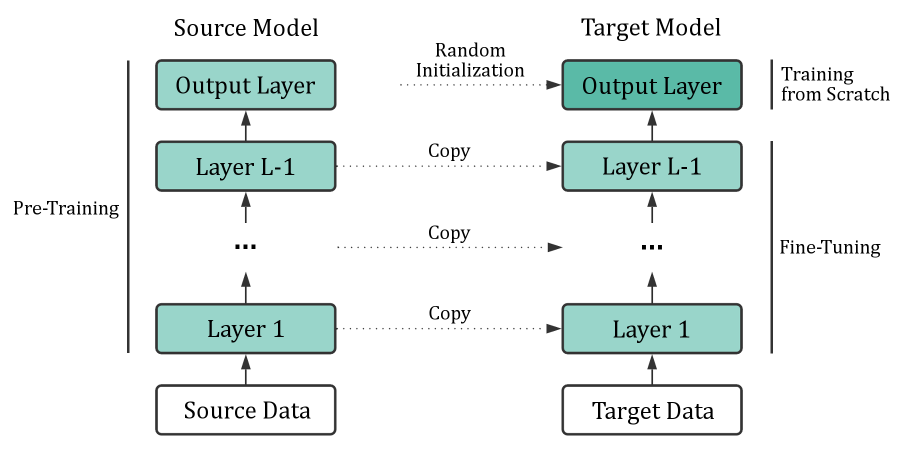
\includegraphics[scale=0.4]{./source/images/finetuning.png}
  \caption{Fine-Tuning vortrainierter Modelle \cite[S.~555]{ZHA20}}
  \label{pic:FineTuning}
\end{figure}

\ac{TL} wird auch in dieser Arbeit genutzt. Einige Komponenten der bereits vorgestellten Architekturen, wie beispielsweise der Encoder oder auch der Decoder, können durch vortrainierte Modelle repräsentiert werden. Hier wird inhaltlich sowie kontextuell in den folgenden Kapiteln angeknüpft, da zunächst die Einführung weiterer \ac{NLP}-Grundlagen erforderlich ist. Die angeführten Vorteile von \ac{TL} können nichtsdestotrotz wie folgt zusammengefasst werden:

\begin{itemize}
	\item Zeitersparnis durch Überspringen des initialen Trainings
	\item Qualitätsanstieg und Generalisierung durch Berücksichtigung massenhafter Daten
	\item Reduktion der hardwaretechnischen Anforderungen und des Stromverbrauches
\end{itemize}
